\chapter{Bouquet for Mom}

The ultimate goal of this project is for the children to create a bouquet for their mothers. When the player clicks on this spot, a beautiful flower will appear. To get the most beautiful bouquet, the player can change the type of flowers using the up arrow. Use the left and right arrows to adjust the size of the flower.

\begin{figure}[H]
   \centering
   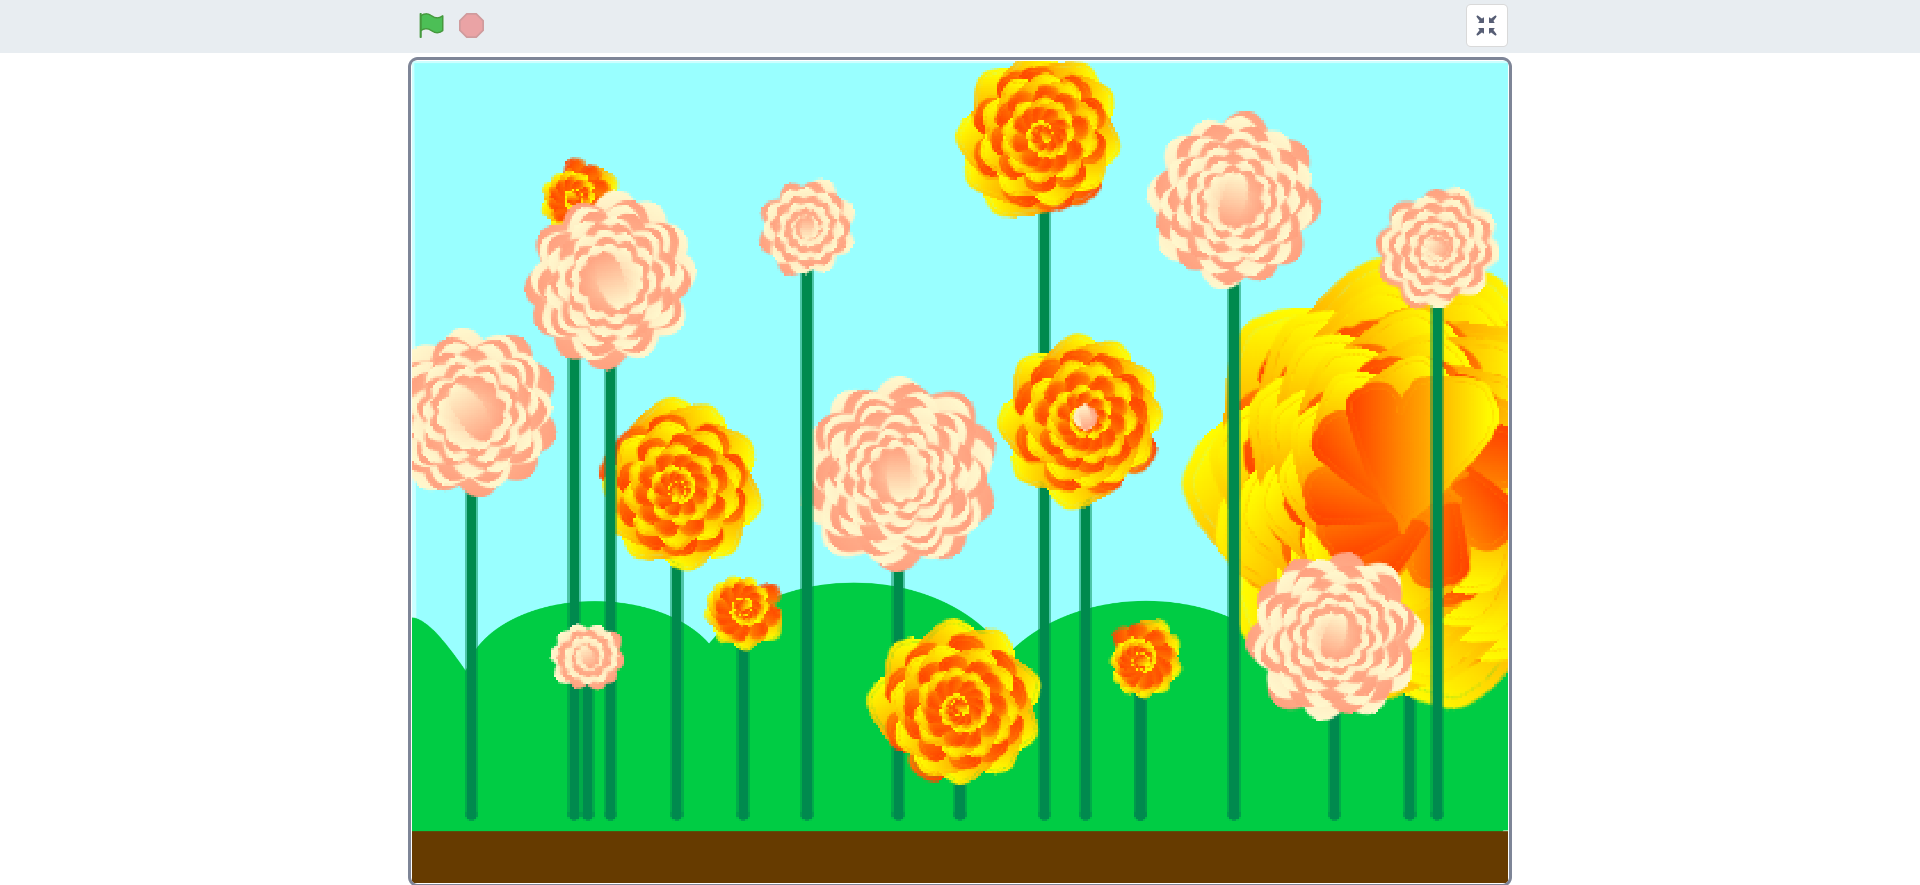
\includegraphics[width=1.0\linewidth,height=0.5\linewidth]{fig040001.png}
   \caption{Bouquet for Mom}
\label{fig040001}
\end{figure}

\section{Adding Background and Characters}
The first step in creating the game is adding a suitable background. From the Backdrops->Choose a Backdrop section. A suitable one can be selected from the available ones that Scratch provides.

In this game, there will be no need for the main character in Scratch the cat. For this, he must be deleted.

\begin{figure}[H]
   \centering
   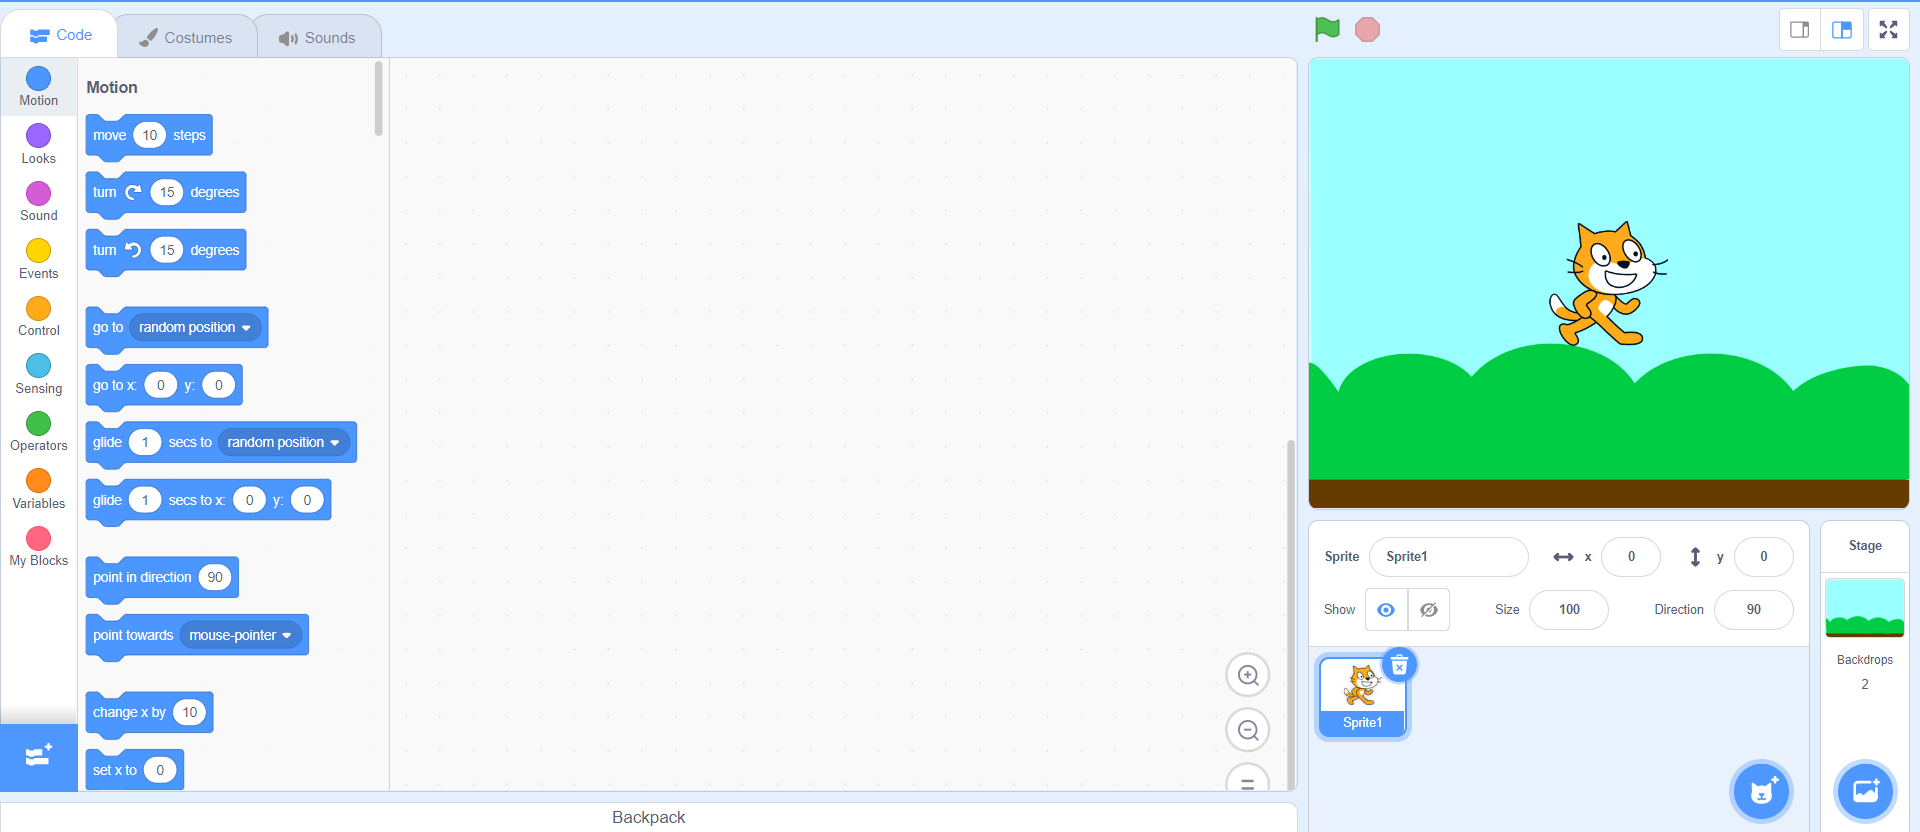
\includegraphics[width=1.0\linewidth,height=0.5\linewidth]{fig040002.png}
   \caption{Game Background}
\label{fig040002}
\end{figure}

The character representing a flower petal created when the player clicks on the screen should be added. This sprite must be drawn using the tools. More than one costume can be added for this character to make the game more interesting. Each of the suits will represent a different petal.

\begin{figure}[H]
   \centering
   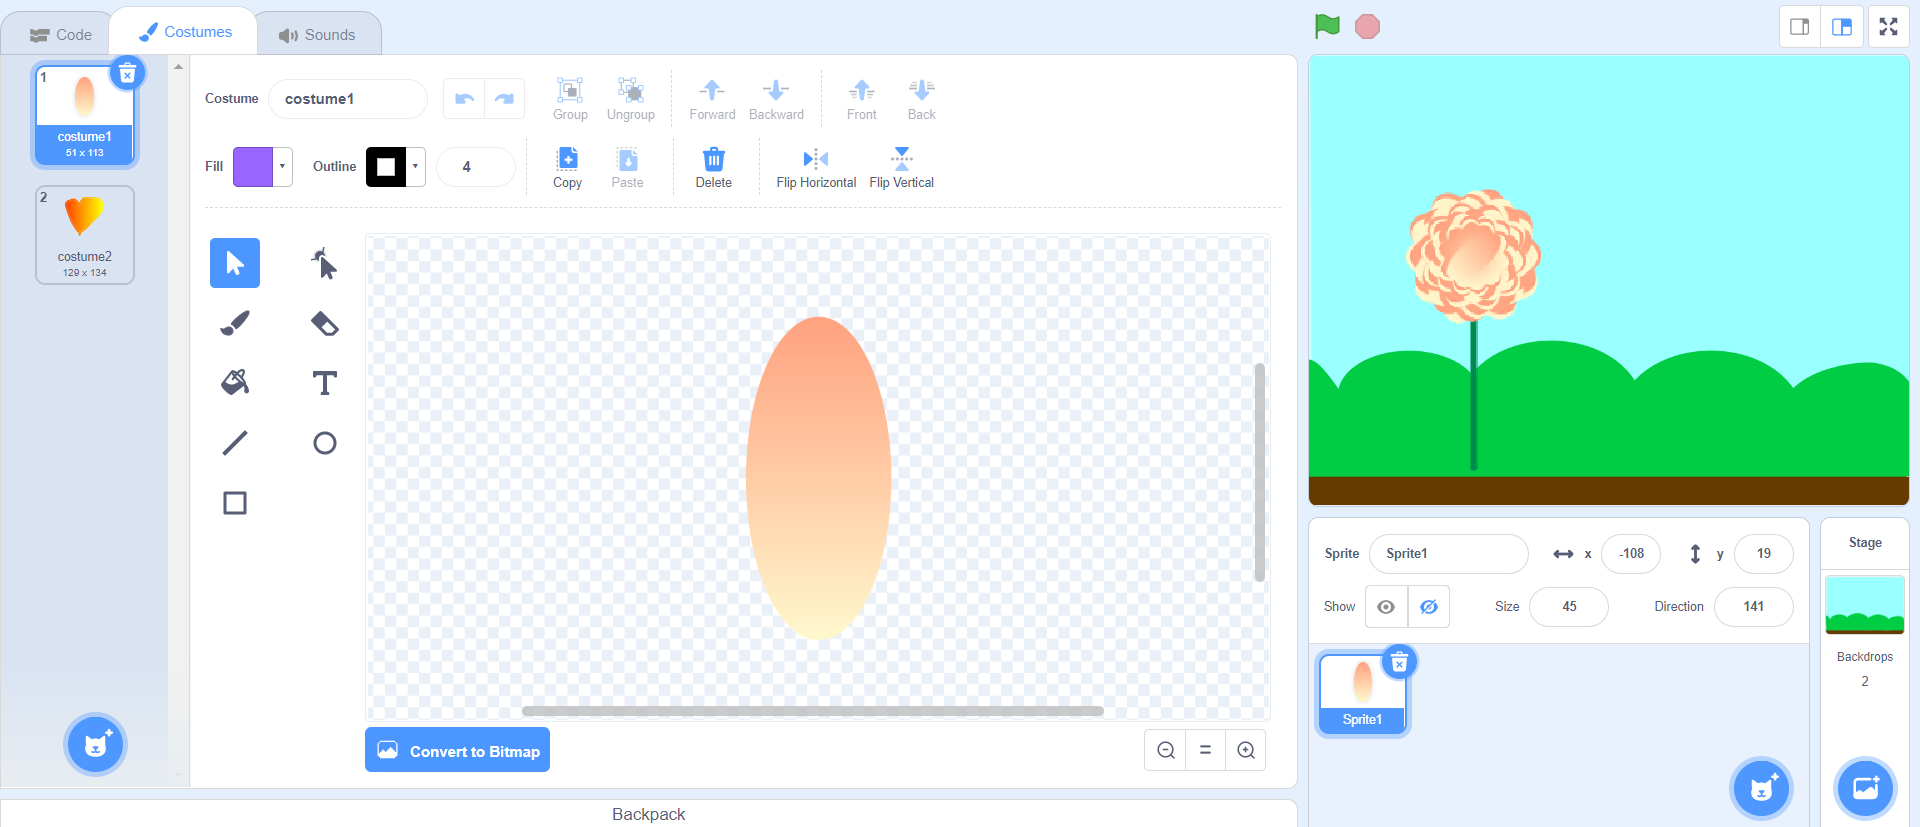
\includegraphics[width=1.0\linewidth,height=0.5\linewidth]{fig040003.png}
   \caption{Drawing Petal Character}
\label{fig040003}
\end{figure}

\section{Drawing Flowers}

When the player clicks on the background, a flower will be drawn. This means that instructions should be placed on the background when clicked to send a "draw" message.

\begin{figure}[H]
   \centering
   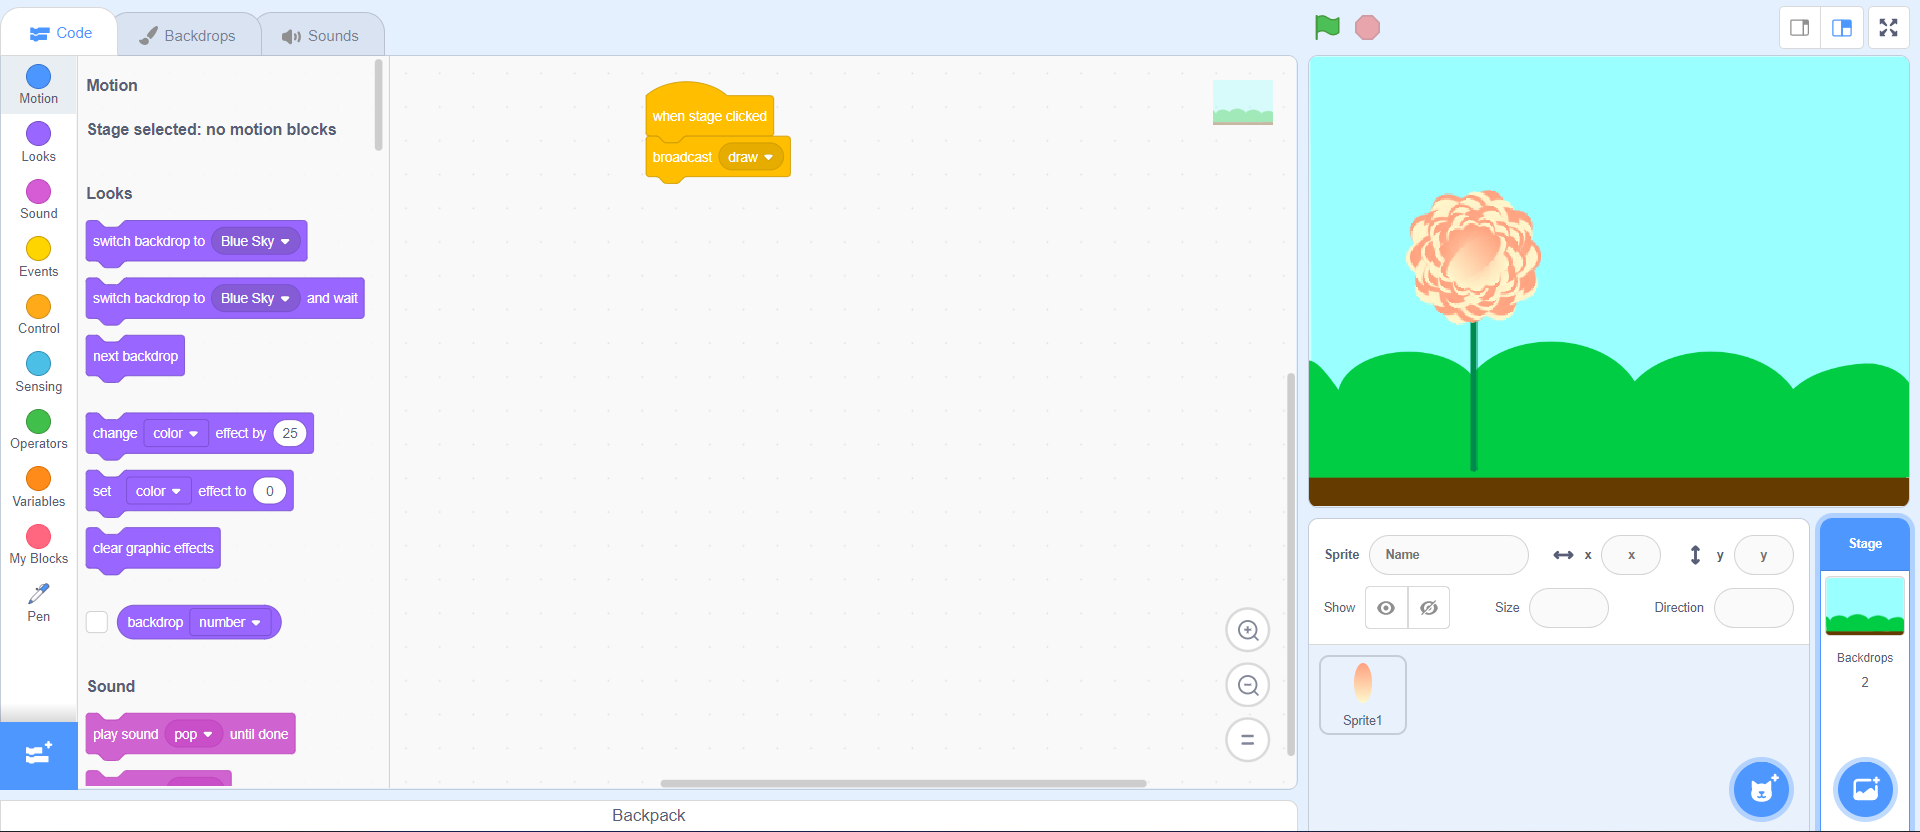
\includegraphics[width=1.0\linewidth,height=0.5\linewidth]{fig040004.png}
   \caption{Background Instructions}
\label{fig040004}
\end{figure}

A new instruction section should be added to draw the flowers and stems. This is the Pen section.

\begin{figure}[H]
   \centering
   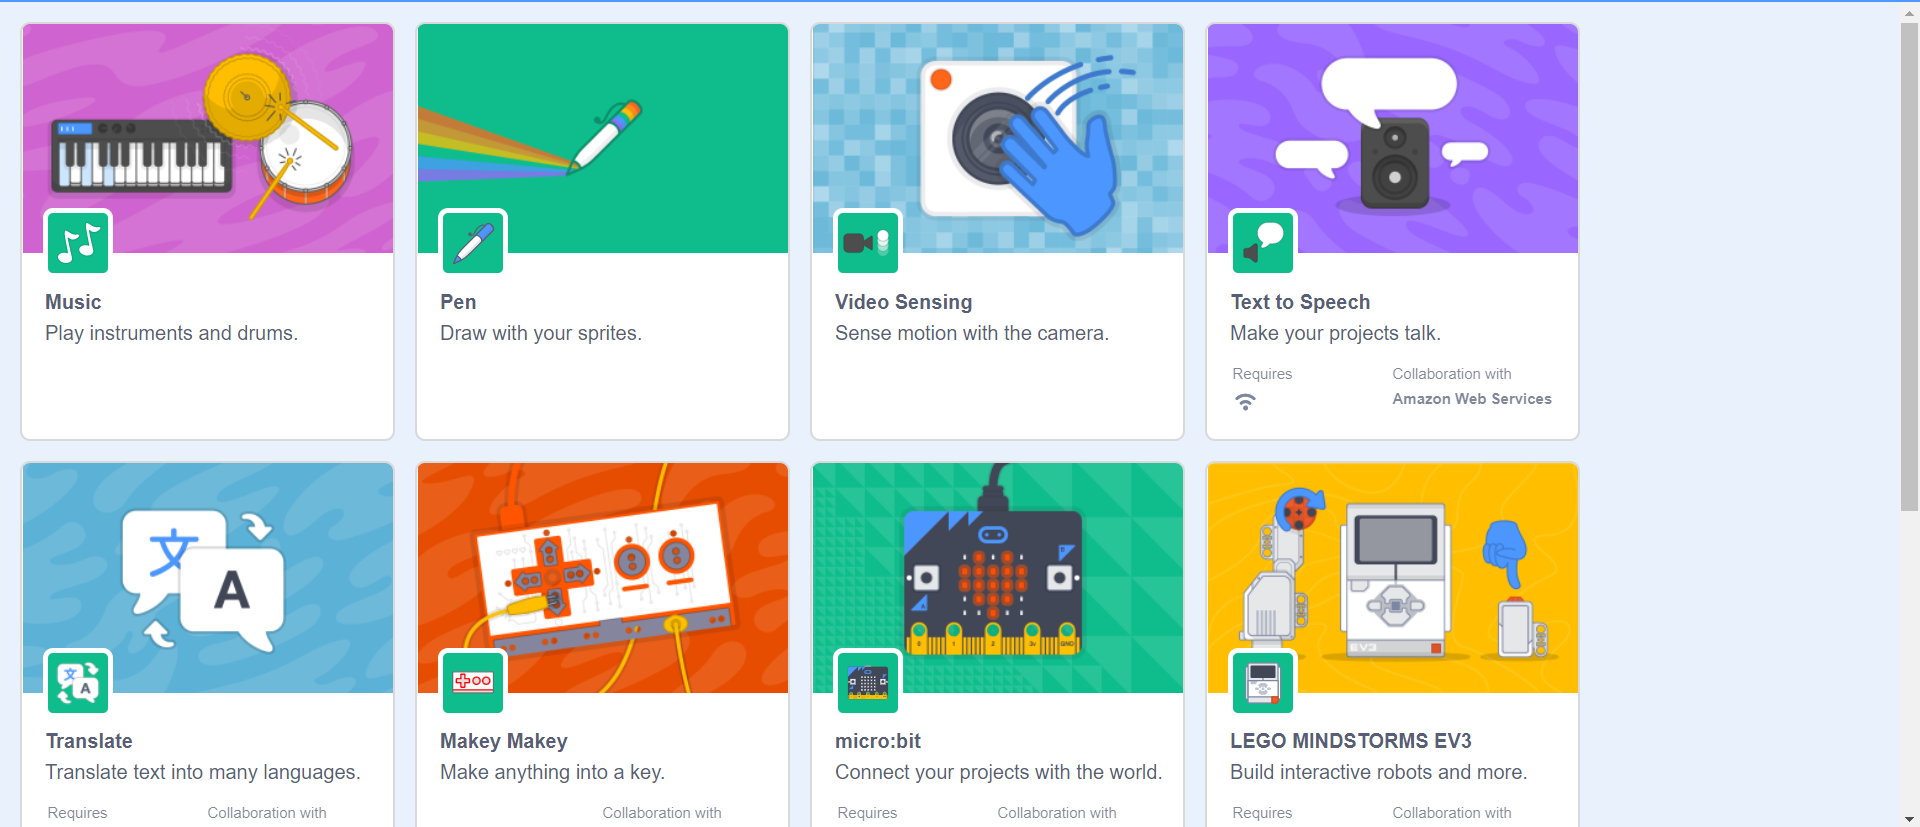
\includegraphics[width=1.0\linewidth,height=0.5\linewidth]{fig040005.png}
   \caption{Add Pen Section}
\label{fig040005}
\end{figure}

When the game starts, the petal character must be hidden, and everything drawn up to that point must be erased. The instruction that erases everything on the screen is located in the new Pen section and is "erase all".

\begin{figure}[H]
   \centering
   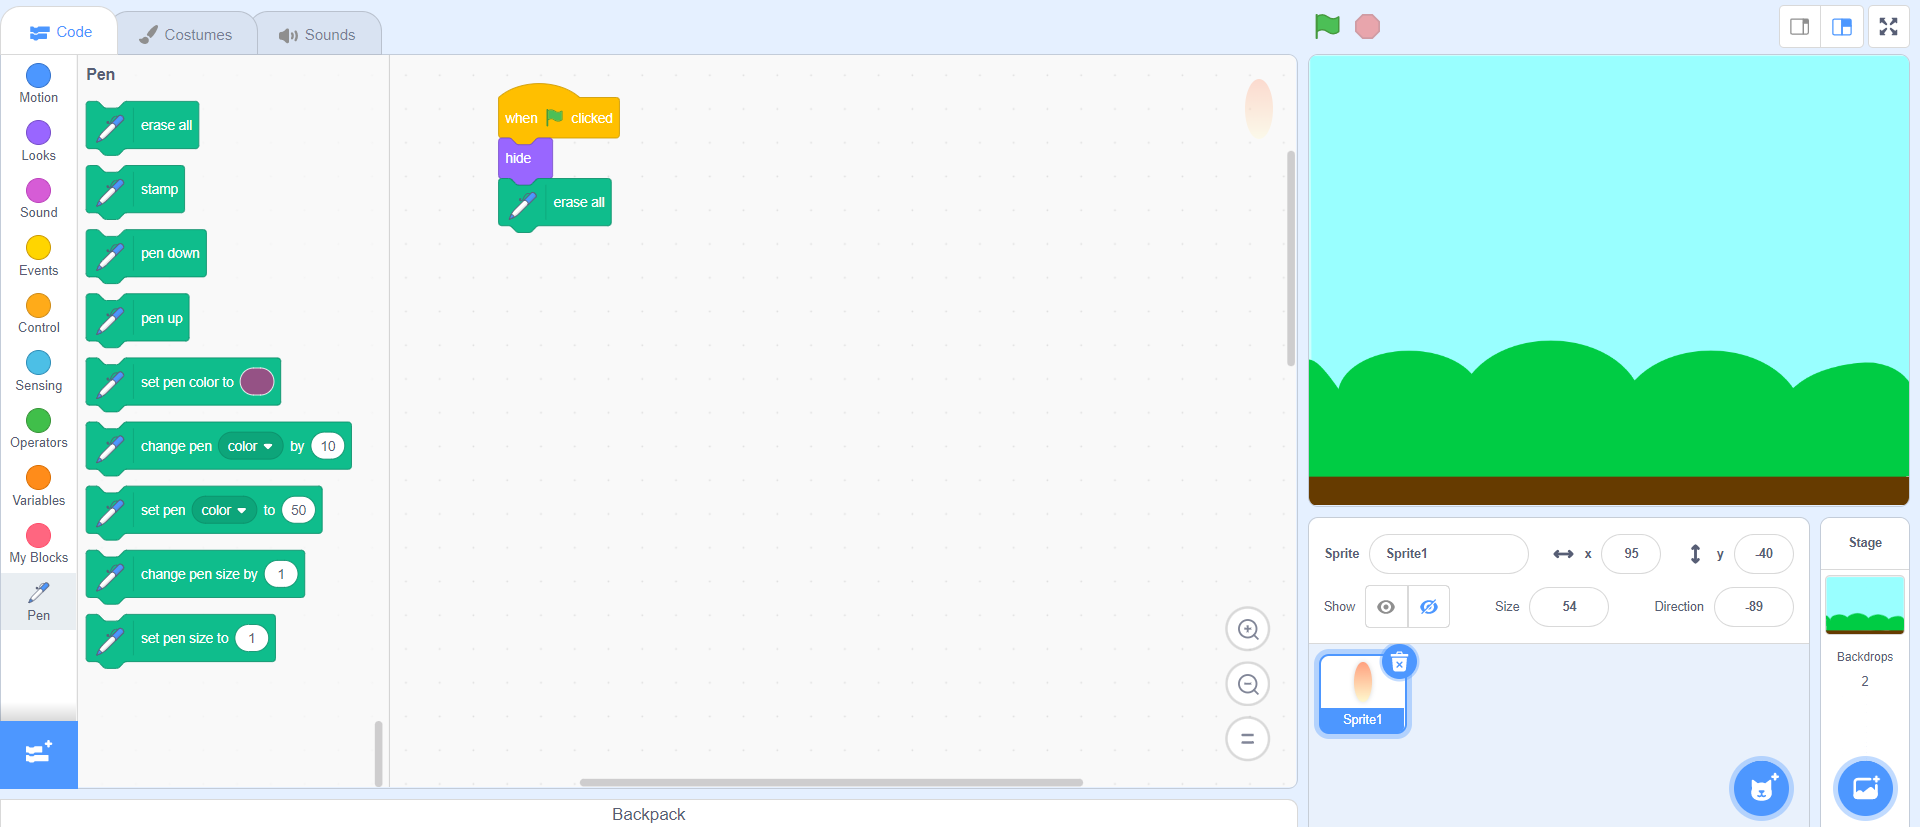
\includegraphics[width=1.0\linewidth,height=0.5\linewidth]{fig040006.png}
   \caption{Start of the game}
\label{fig040006}
\end{figure}

Before drawing the flower itself, its companion will be drawn first. Drawing the handle will start when the "draw" message is received. First, the thickness of the pencil that will be drawn and the color will be set. First, the pencil must be positioned. The initial x coordinate is the same as the mouse's. The instruction in the light blue group gives the mouse position for x. The initial y coordinate should be -150. Once the character is positioned, the pencil should be instructed to come down to start drawing. To complete the flower's stem, the character must go to where the mouse is and pick up the pencil.

The result of the following code (Fig. \ref{fig040007}) is that the flower will be drawn when the player clicks on different places on the screen.

\begin{figure}[H]
   \centering
   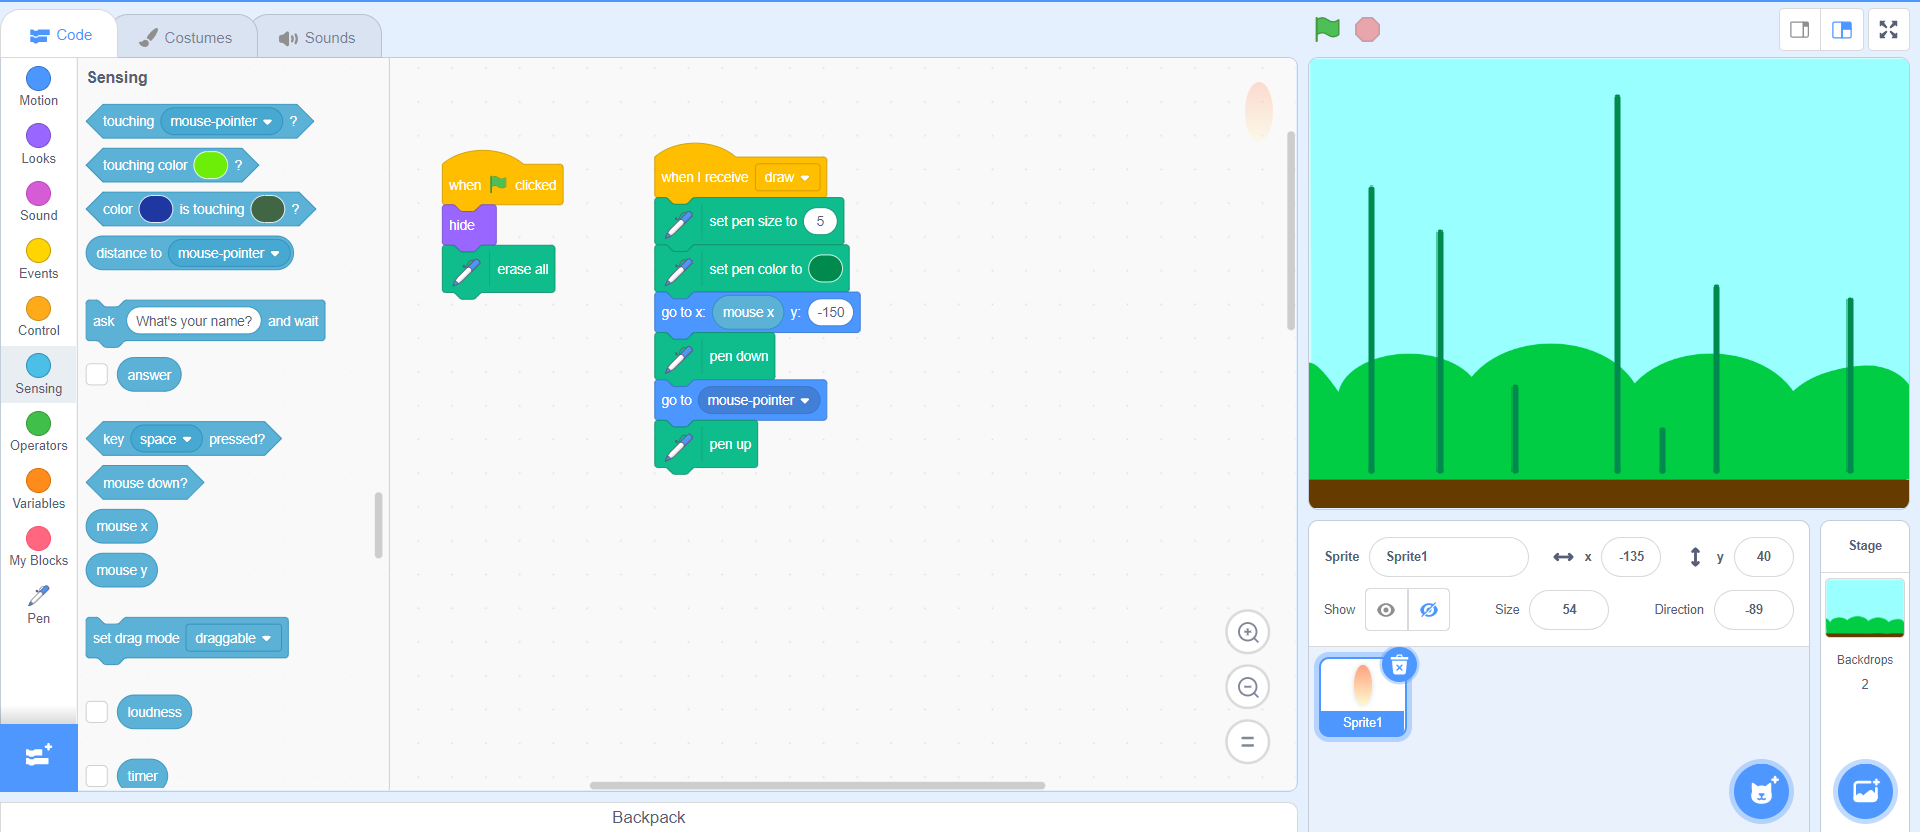
\includegraphics[width=1.0\linewidth,height=0.5\linewidth]{fig040007.png}
   \caption{Drawing the flower stems}
\label{fig040007}
\end{figure}

The drawn character must leave traces, like a stamp, to get the flower. Each time it leaves a trail, it must rotate and decrease its size by one. This algorithm must be repeated. In this way, the effect of the flowers is achieved. To obtain different flowers, the iterations of the drawing algorithm will be a random number between 40 and 60.

\begin{figure}[H]
   \centering
   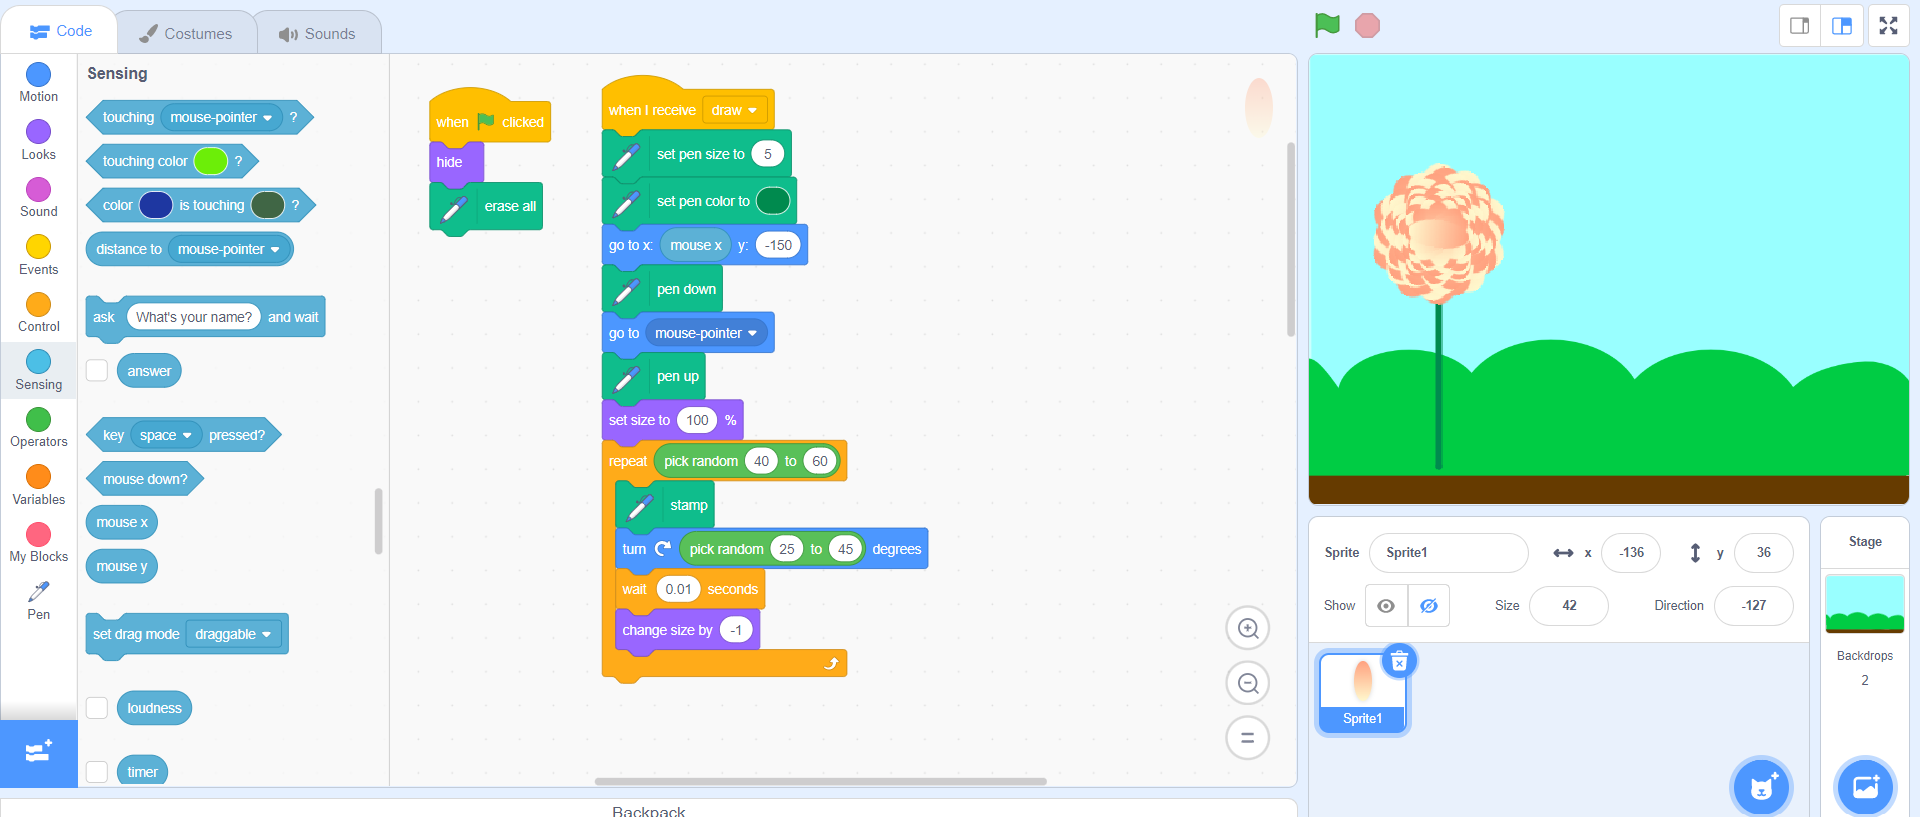
\includegraphics[width=1.0\linewidth,height=0.5\linewidth]{fig040008.png}
   \caption{Drawing the flowers}
\label{fig040008}
\end{figure}

The result so far is that when the player clicks on different places on the screen, the flowers for mom will appear.

\section{Changing the type and size of flowers}

To make the game more interesting, using the up arrow will change the character's costumes. So the more suits there are, i.e., the more petals there are, the more diverse the bouquet will be.

\begin{figure}[H]
   \centering
   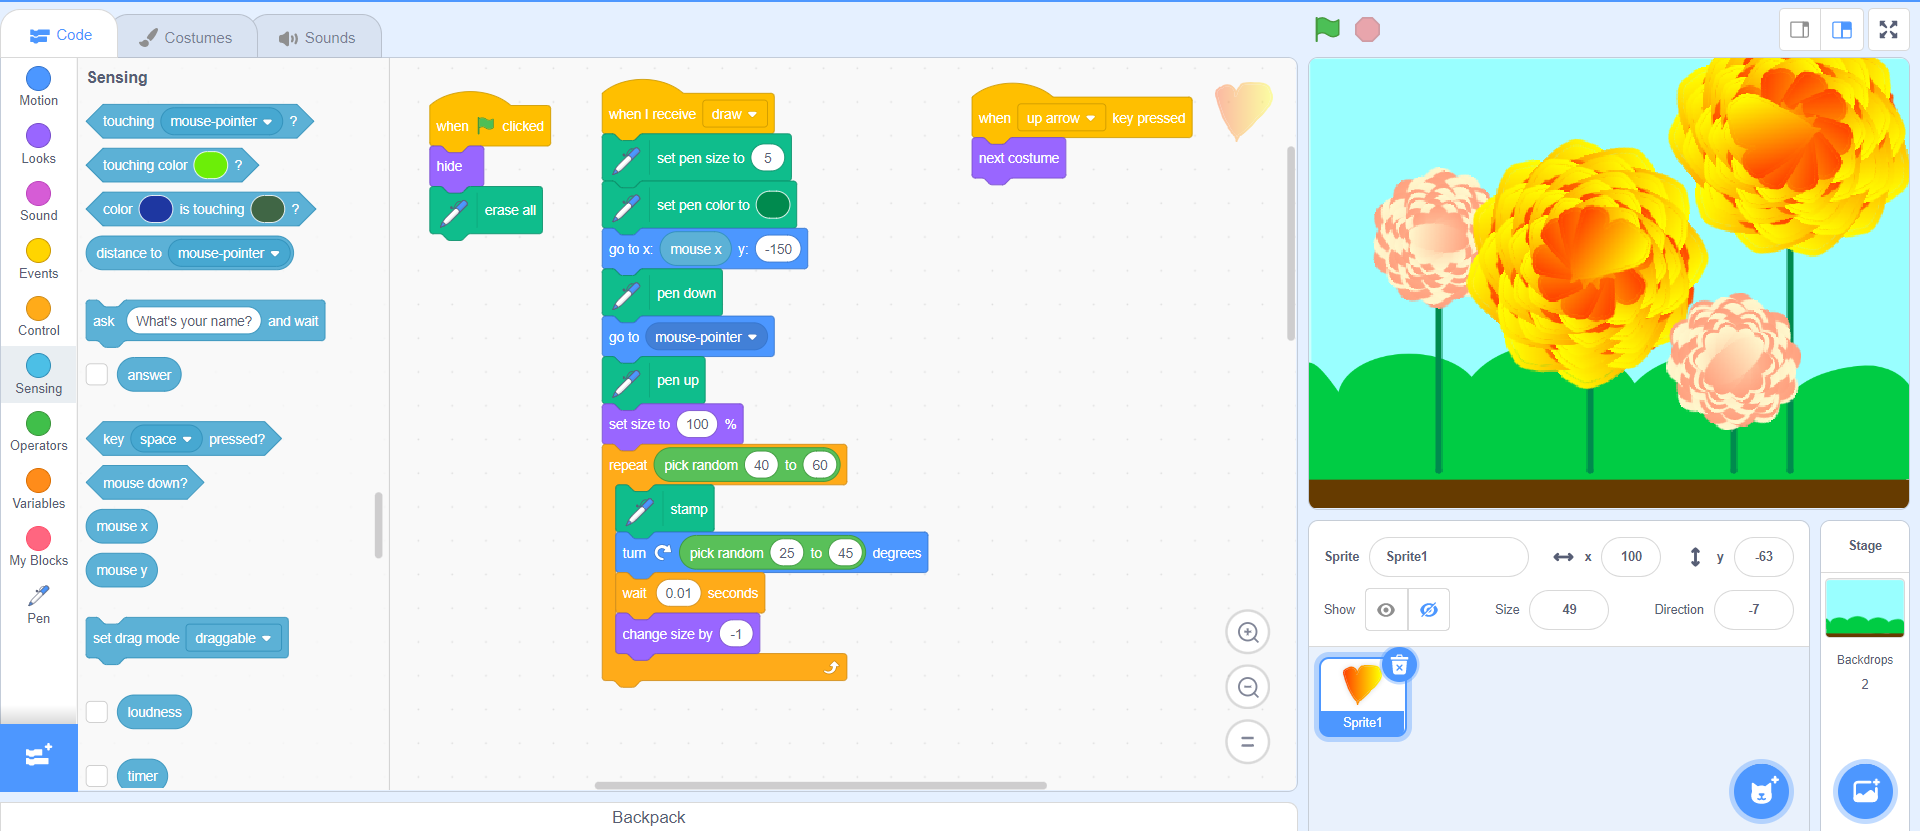
\includegraphics[width=1.0\linewidth,height=0.5\linewidth]{fig040009.png}
   \caption{Character Costume Changes}
\label{fig040009}
\end{figure}

Another improvement that can be made is to change the size of the flowers. For this purpose, the first thing to be done is a variable to hold the character's size. A characteristic of variables is that they have an initial value, and that value can be changed. In this case, the initial value of the variable will be 100. Pressing the left arrow will decrease the variable by 10, and pressing the right arrow will increase the variable by 10. This is what the final program code looks like:

\begin{figure}[H]
   \centering
   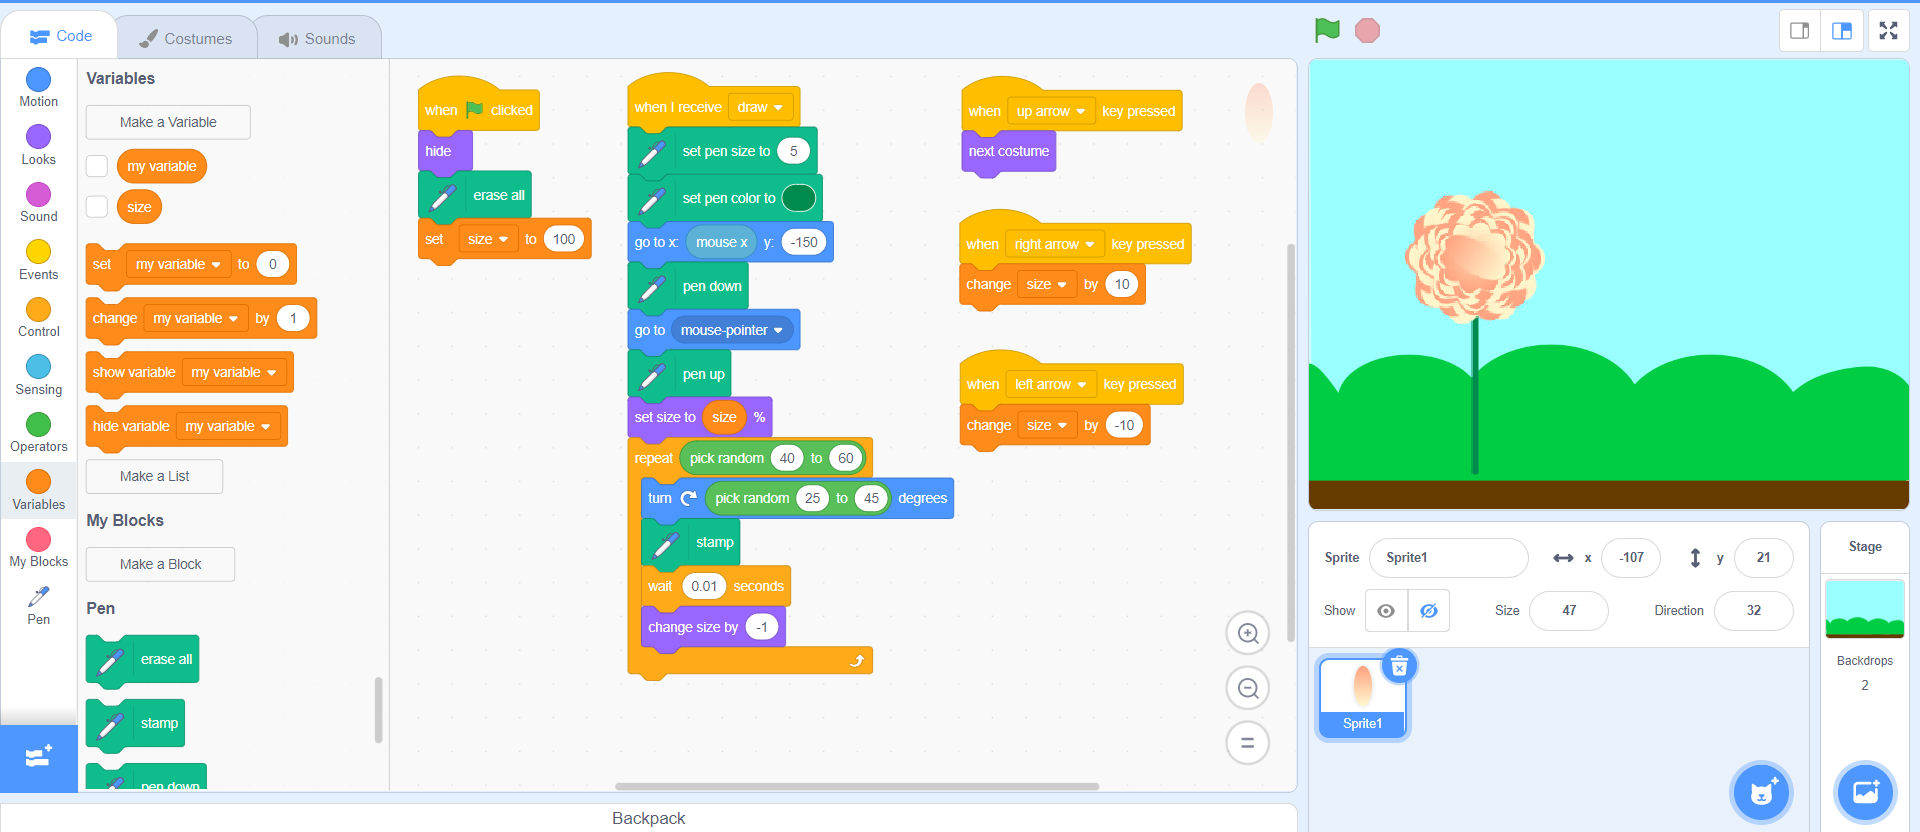
\includegraphics[width=1.0\linewidth,height=0.5\linewidth]{fig040010.png}
   \caption{Full program code}
\label{fig040010}
\end{figure}

The children must present the most beautiful bouquet to their mothers!
